% File SDSS2020_SampleExtendedAbstract.tex
\documentclass[10pt]{article}\usepackage[]{graphicx}\usepackage[table]{xcolor}
% maxwidth is the original width if it is less than linewidth
% otherwise use linewidth (to make sure the graphics do not exceed the margin)
\makeatletter
\def\maxwidth{ %
  \ifdim\Gin@nat@width>\linewidth
    \linewidth
  \else
    \Gin@nat@width
  \fi
}
\makeatother

\definecolor{fgcolor}{rgb}{0.345, 0.345, 0.345}
\newcommand{\hlnum}[1]{\textcolor[rgb]{0.686,0.059,0.569}{#1}}%
\newcommand{\hlstr}[1]{\textcolor[rgb]{0.192,0.494,0.8}{#1}}%
\newcommand{\hlcom}[1]{\textcolor[rgb]{0.678,0.584,0.686}{\textit{#1}}}%
\newcommand{\hlopt}[1]{\textcolor[rgb]{0,0,0}{#1}}%
\newcommand{\hlstd}[1]{\textcolor[rgb]{0.345,0.345,0.345}{#1}}%
\newcommand{\hlkwa}[1]{\textcolor[rgb]{0.161,0.373,0.58}{\textbf{#1}}}%
\newcommand{\hlkwb}[1]{\textcolor[rgb]{0.69,0.353,0.396}{#1}}%
\newcommand{\hlkwc}[1]{\textcolor[rgb]{0.333,0.667,0.333}{#1}}%
\newcommand{\hlkwd}[1]{\textcolor[rgb]{0.737,0.353,0.396}{\textbf{#1}}}%
\let\hlipl\hlkwb

\usepackage{framed}
\makeatletter
\newenvironment{kframe}{%
 \def\at@end@of@kframe{}%
 \ifinner\ifhmode%
  \def\at@end@of@kframe{\end{minipage}}%
  \begin{minipage}{\columnwidth}%
 \fi\fi%
 \def\FrameCommand##1{\hskip\@totalleftmargin \hskip-\fboxsep
 \colorbox{shadecolor}{##1}\hskip-\fboxsep
     % There is no \\@totalrightmargin, so:
     \hskip-\linewidth \hskip-\@totalleftmargin \hskip\columnwidth}%
 \MakeFramed {\advance\hsize-\width
   \@totalleftmargin\z@ \linewidth\hsize
   \@setminipage}}%
 {\par\unskip\endMakeFramed%
 \at@end@of@kframe}
\makeatother

\definecolor{shadecolor}{rgb}{.97, .97, .97}
\definecolor{messagecolor}{rgb}{0, 0, 0}
\definecolor{warningcolor}{rgb}{1, 0, 1}
\definecolor{errorcolor}{rgb}{1, 0, 0}
\newenvironment{knitrout}{}{} % an empty environment to be redefined in TeX

\usepackage{alltt}
\usepackage{sdss2020} % Uses Times Roman font (either newtx or times package)
\usepackage{url}
\usepackage{latexsym}
\usepackage{amsmath, amsthm, amsfonts}
\usepackage{algorithm, algorithmic}  
\usepackage{graphicx}
\usepackage[table]{xcolor}
\usepackage{caption}

\usepackage{titlesec}
\setlength{\belowcaptionskip}{-15pt}
\usepackage{parskip}
\setlength{\parskip}{0.2\baselineskip plus 1pt}

\title{Testing statistical charts for accuracy and interpretation}

\author{Anonymous}
% \author{
%  Kiegan Rice \\
%   Affiliation / Address line 1  \\
%   Affiliation / Address line 2  \\
%   {\tt email@domain} \\\And
%   Heike Hofmann \\
%   Department of Statistics  \\
%   Iowa State University  \\
%   {\tt hofmann@iastate.edu} \\\And
%   Nola du Toit \\
%   Affiliation / Address line 1  \\
%   Affiliation / Address line 2  \\
%   {\tt email@domain} \\\And
%   Edward Mulrow \\
%   Affiliation / Address line 1  \\
%   Affiliation / Address line 2  \\
%   {\tt email@domain} \\}
\IfFileExists{upquote.sty}{\usepackage{upquote}}{}
\begin{document}
\titlespacing{\subsection}{0pt}{1ex}{0ex}
\titlespacing{\section}{0pt}{1ex}{0ex}

%\titlespacing*{\section} {0pt}{3.5ex plus 1ex minus .2ex}{2.3ex plus .2ex}
%\titlespacing*{\subsection} {0pt}{3.25ex plus 1ex minus .2ex}{1.5ex plus .2ex}

\maketitle
% \begin{abstract}
% The use of visuals is a key component in scientific communication, and decisions about the design of a data visualization should be informed by what design elements best support the audience's ability to perceive and understand the components of the data visualization. We build on the foundations of Cleveland and McGill's work in graphical perception \cite{cleveland}, employing a large, nationally-representative, probability-based panel of survey respondents to test perception in statistical charts. Our findings provide actionable guidance for data visualization practitioners to employ in their work. 
% \end{abstract}

{\bf Keywords:} Graphical Perception, Data Visualization, Scientific Communication

\section{Introduction}

%Why is it important that graphics are good? 
Communication of scientific results to the general public is essential. The use of visuals is a key component in scientific communication; visuals can help provide context, explain scientific concepts, highlight findings, and display patterns in data. 

Decisions about the design of a data visualization are made by the author, and may be driven by subject matter conventions, branding choices, or personal style preferences. When used to communicate with the general public, choices about data visualizations should be informed by knowledge on what best supports the audience in understanding the data and conclusions correctly. %We want  choices about data visualizations to be informed by knowledge on what best supports the statement in the data. 

%We distinguish between two components of audience understanding: perception and cognition. Being able to accurately read information from a chart (perception) is a crucial first step and the basis to enable the second state -- connecting the individual pieces of information from the chart to a connected whole of insight about the data (cognition).  


Cleveland and McGill~\shortcite{cleveland} proposed a list of basic graphical perception tasks and experimentally determined an accuracy-based ranking of those tasks. This ranking has been reproduced by others~\cite{heer}. The tasks proposed by Cleveland and McGill involve assessments of elementary chart elements which focus solely on the \textit{structural} components of a chart: the mapping of a statistical quantity to a particular shape, size, and position in an image. These studies do not address the impact of \textit{aesthetics} on perception: orientation of elements in a chart, context provided, color mappings, and supporting visual elements such as borders, labels, and reference or grid lines. 

Cleveland and McGill recruited colleagues and their spouses for their evaluation, while the Heer study used respondents to Amazon Mechanical Turk\footnote{https://www.mturk.com/}. 

We extended the tasks proposed by Cleveland and McGill to complete a series of tests on graphical perception in modern data visualization, incorporating and varying both structural and aesthetic elements within the charts presented to viewers. In addition, we utilized a nationally-representative sample of U.S. adults to better understand how the general public as a whole perceives graphics, in contrast to the convenience samples used by prior studies.  
%("We analyzed a total of 2,880 responses from the two experimental runs" HH: not sure how many participants that corresponds to). 

%KR: here are the citations
%\cite{cleveland}, \cite{heer}, \cite{lu2021jnd}, 
%\cite{skau}, \cite{eells}, \cite{vonHuhn}, \cite{spence}

%Overview by  Tableau researchers: https://research.tableau.com/sites/default/files/bar.pdf



\section{Methods}

We conducted a series of tests focusing on the public's ability to perceive differences between two values displayed in a chart. Each test asked the respondents to identify which of two elements displayed in a chart was larger. We varied the \textit{structure} of the visual elements as well as the \textit{aesthetics} used in the chart. 

\subsection{Test population}

We employ AmeriSpeak's Omnibus\footnote{https://amerispeak.norc.org/us/en/amerispeak/our-capabilities/amerispeak-omnibus.html} survey, which utilizes a probability-based panel and surveys a sample of 1,000 nationally representative adults 18 and older. The advantage of using probability-based panel approach is two-fold. First, we have access to a large sample of survey participants and thus have greater power in making inference about graphical perception abilities. Second, the sample is representative of the general adult public in the U.S., which is an important target audience for scientific communication. 

In some rounds, respondents were split into two groups and each group received a different stimulus; each stimulus in every round was seen and responded to by at least 465 respondents. %\textbf{OVER 400 RESPONDENTS -- DO WE HAVE THE ACTUAL MIN HANDY?}. HH: round 1, colors were evaluated by 465.


\subsection{Test stimulus}

\begin{figure*}
\centering
\begin{tabular}{lll}
(a) vertical & (b) horizontal & (c) horizontal wide \\
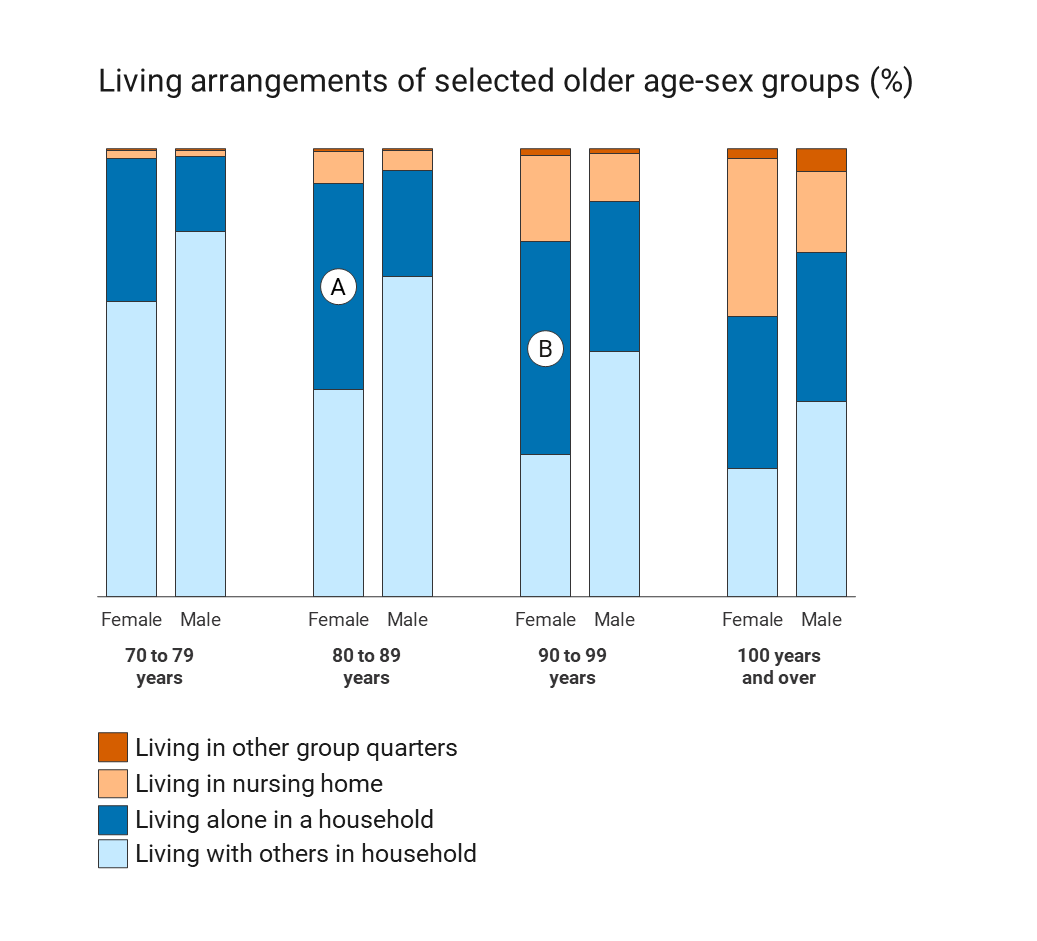
\includegraphics[width=0.25\textwidth]{images/vertical.PNG} &
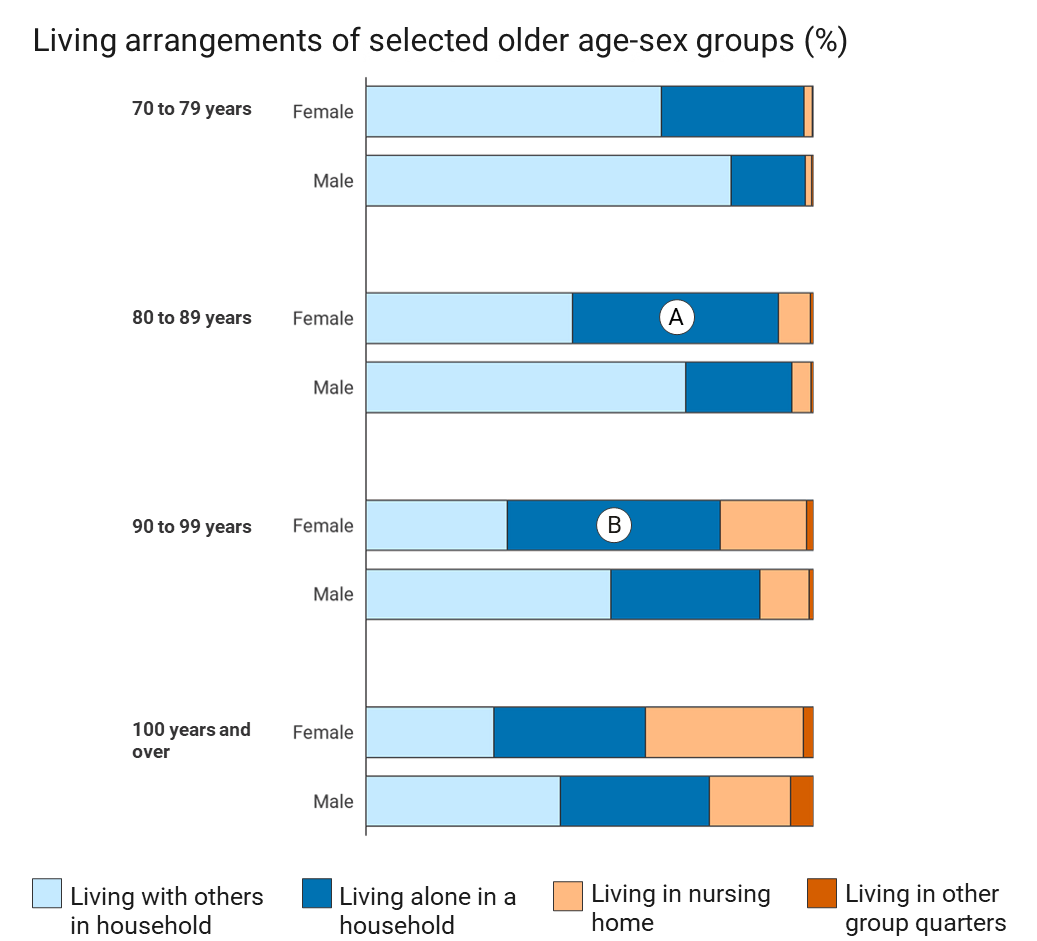
\includegraphics[width=0.25\textwidth]{images/horizontal.PNG} &
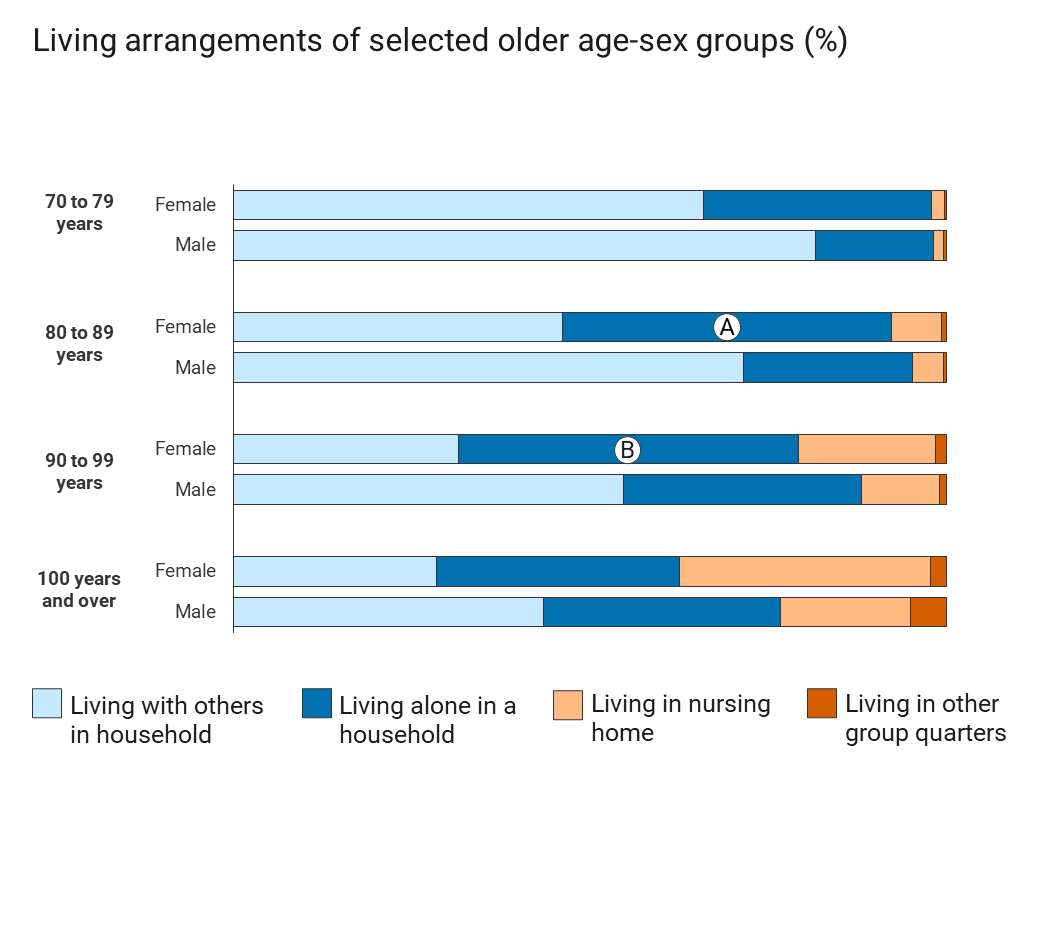
\includegraphics[width=0.25\textwidth]{images/horizontal-wide.PNG} 
\end{tabular}
\caption{\label{stimulus} From left to right three stacked barcharts shown to panelists. The difference in value between A and B is the same throughout all charts (B is larger). The area of the representation is kept constant; the difference in heights/widths between bars A and B changes from 7 pixels in (a) and (b) to 11 pixels in (c). }
\end{figure*}

The tasks focused on determining which of two very similar values were larger. The two values were chosen close to the \textit{just noticeable difference} (the theoretical difference for which about half of the population is able to determine the difference correctly), making this a visually hard task at the boundary of our perception \cite{lu2021jnd}. Our assumption is that even small changes to this task can have a large effect on a viewer's perception resulting in measurable changes of the overall accuracy.  %Respondents could also select the option that the values were the same. \textbf{KR: WE SHOULD NOTE IN RESULTS SECTION RESULTS ARE CONSISTENT EITHER WAY, OR CUT THIS SENTENCE IN THE ABSTRACT.} 

Values were depicted as pieces of a stacked bar chart, shown in Figure~\ref{stimulus}. Responses were collected from a series of variations to structure and aesthetics. Differences in structure included whether the marked pieces were aligned along a common baseline or not, as well as the orientation of the chart as a horizontal or vertical stacked bar chart (see Figure~\ref{stimulus}a,b). Differences in aesthetics included variations in the color scheme used, use of grid lines, and removal of all relevant context (not shown). 
%
\section{Results}
Each one of the stacked barcharts in Figure~\ref{stimulus} was shown to panelists in two versions: with bars A and B aligned along a common axis and the stacked version shown in the image.  The results of these evaluations are shown in Figure~\ref{fig:aligned}. Like Cleveland and McGill, we find that assessing the difference between aligned bars is easier than between unaligned bars (McNemar test statistic 372.15, $p$-value = $2.2 \times 10^{-16}$).

\begin{figure}
\centering
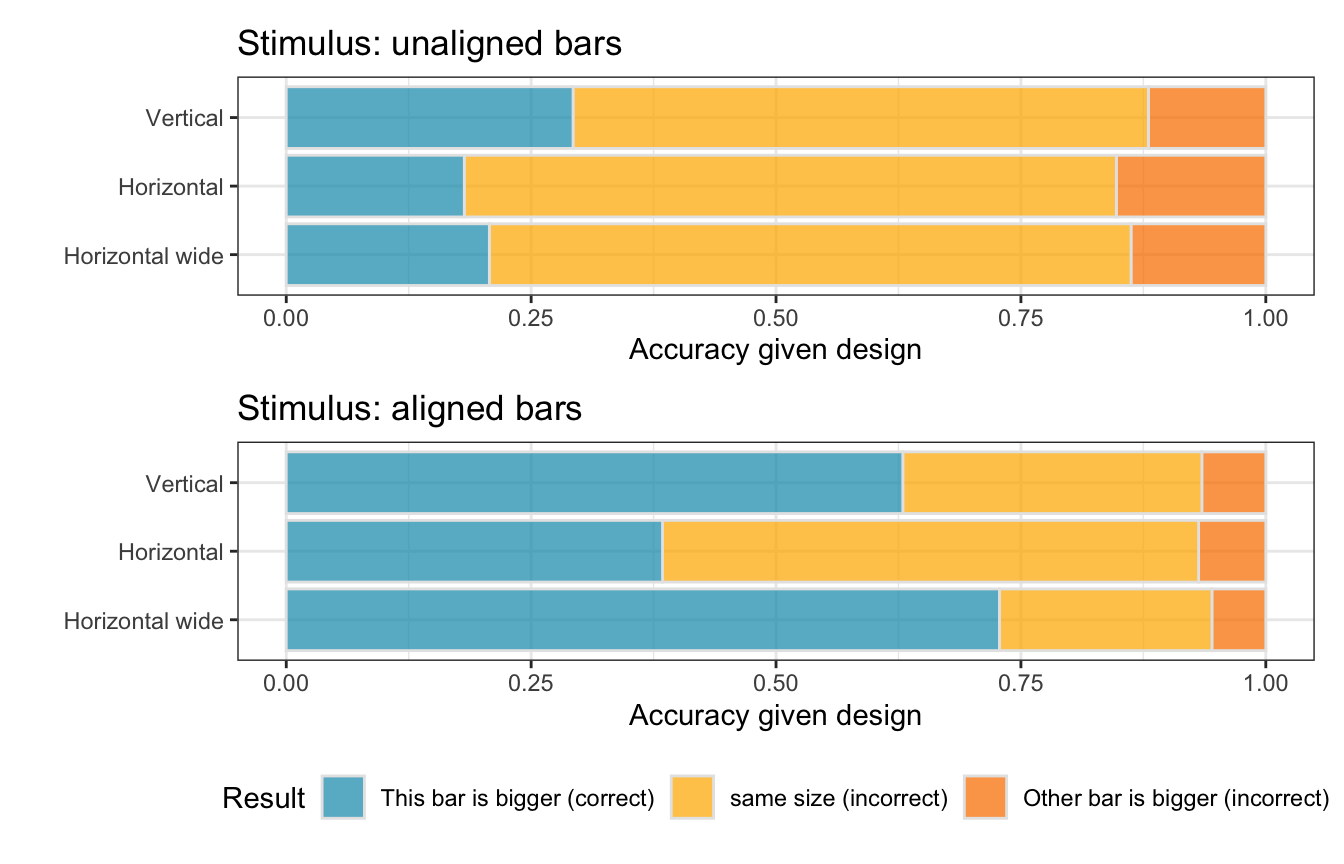
\includegraphics[width=\columnwidth]{images/fig-aligned-round4-1.png}
\caption{\label{fig:aligned} A large number of respondents chose the answer 'the bars are the same size'. While correct for the purposes of interpretation, technically this answer is not the most accurate. Differences between aligned bars are correctly identified at about twice the rate of stacked bars. }
\end{figure}
The design choices are clearly having an impact on accuracy. The change from a horizontal to a vertical design leads to a significant loss in accuracy for both aligned and stacked bars. 
The re-scaled design of the wide horizontal bars reclaims some of the loss for stacked bars and outperforms the vertical design by a similar margin in aligned bars. 
This improves performance of the wide horizontal design over the horizontal design is expected: bars are overall wider and closer together, both factors positively affect accuracy \cite{lu2021jnd}.

\begin{figure}
\centering
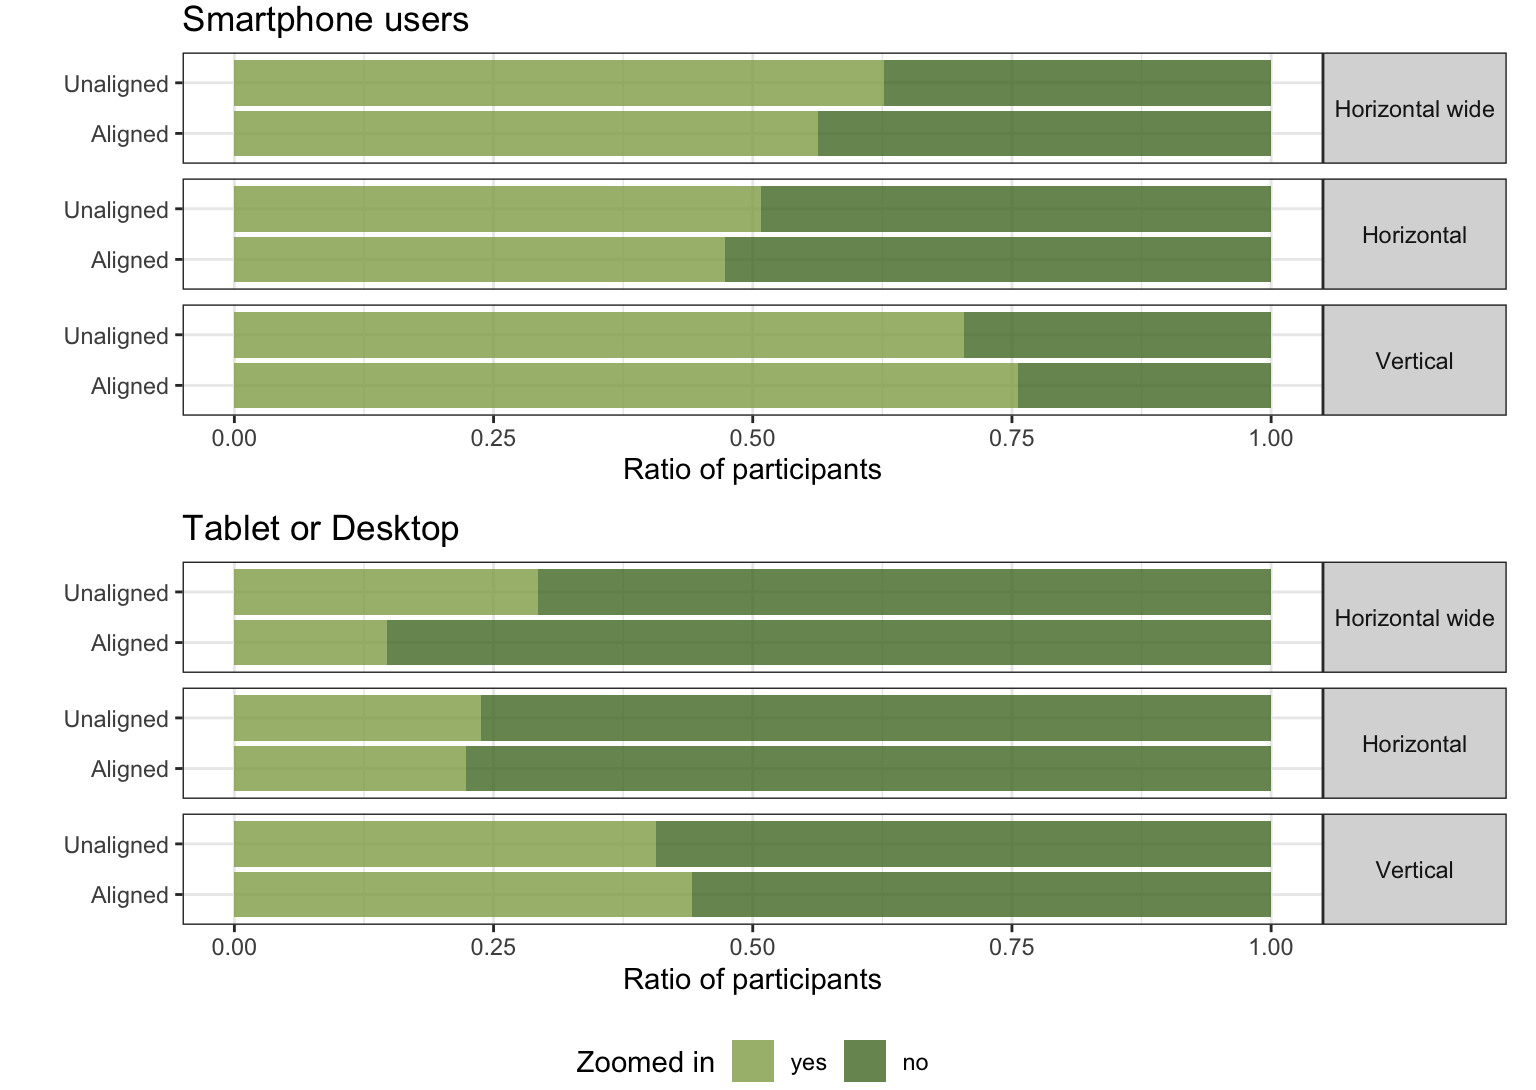
\includegraphics[width=\columnwidth]{images/zoomers3-1.png}
\caption{\label{zooming}Devices with small screens lead to about twice the zooming rate as tablets or desktops. Panelists zoom into the vertical design, but less so into horizontal designs.}
\end{figure}

Another factor contributing to the difference in accuracy between the vertical and the horizontal is how participants interact with the different designs: generally, about half of all participants make use of the option to zoom into charts (which improves accuracy by about 5 percentage points on average).  Figure~\ref{zooming} shows that zooming behavior of panelists changes depending on the design of the chart. 

\section{Conclusions/Further Work}
We have shown that the format of the AmeriSpeak panel allows us to reproduce findings established in the literature.  This provides us with a unique opportunity to create an experimentally validated portfolio of graphical insights:
Grid lines improve accuracy in comparisons, isolating the visual task from its context in the chart seems oddly detrimental to an accurate assessment, forcing panelists to rank objects by size (rather than offering the choice of 'same') does not change the relative rate between the other choices, but increases time spent on an evaluation and reduces certainty in one's response. 
%
\vspace{-10pt}
\bibliographystyle{sdss2020} % Please do not change the bibliography style
\bibliography{references}
\end{document}
